% =====================================================================
\chapter{Metodologi Penelitian}
\label{bab:3}
% =====================================================================
Bab ini membahas metodologi penelitian yang meliputi tahapan penelitian, pengumpulan data, analisis kebutuhan, perancangan sistem, implementasi, pengujian dan evaluasi, serta jadwal penelitian.

% ---------------------------------------------------------------------
\section{Tahapan Penelitian}
\label{sec:tahapan}
Penelitian ini menggabungkan pengembangan perangkat lunak dengan eksperimen terhadap mesin RAG. Tahapan pengembangan mengikuti model \textit{waterfall} yang terdiri atas analisis kebutuhan, perancangan, implementasi, dan pengujian \parencite{sommerville2016software}, dengan tambahan tahap evaluasi kualitas jawaban. Tahapan penelitian ditunjukkan pada Gambar~\ref{fig:tahapan}.

\begin{figure}[htbp]
\centering
\begin{tikzpicture}[font=\normalsize, node distance=0.55cm,
  term/.style={draw, rounded rectangle, minimum width=3.2cm, minimum height=0.9cm, align=center},
  proc/.style={draw, rectangle, minimum width=7.4cm, minimum height=0.95cm, align=center, text width=7.2cm},
  dec/.style={draw, diamond, aspect=2.6, align=center, inner sep=1pt},
  io/.style={draw, trapezium, trapezium left angle=72, trapezium right angle=108, minimum height=0.9cm, align=center, text width=3.4cm},
  arr/.style={-{Stealth[length=2mm]}, thick}]
\node[term] (mulai) {Mulai};
\node[proc, below=of mulai] (lit) {Studi literatur dan analisis sistem sejenis};
\node[io, below=of lit, text width=5.6cm] (data) {Pengumpulan data: 7 SOP, wawancara staf, benchmark 40 pertanyaan};
\node[proc, below=of data] (keb) {Analisis kebutuhan fungsional dan nonfungsional};
\node[proc, below=of keb] (ran) {Perancangan: arsitektur, graf alur kerja, alur LangGraph, API, basis data};
\node[proc, below=of ran] (imp) {Implementasi mesin \wgr{} dan integrasi E-Office};
\node[proc, below=of imp] (uji) {Pengujian \textit{black-box} dan evaluasi kualitas jawaban};
\node[dec, below=of uji] (ok) {Memenuhi\\kebutuhan?};
\node[proc, below=0.6cm of ok] (lap) {Analisis hasil dan penyusunan laporan};
\node[term, below=of lap] (selesai) {Selesai};
\draw[arr] (mulai)--(lit); \draw[arr] (lit)--(data); \draw[arr] (data)--(keb);
\draw[arr] (keb)--(ran); \draw[arr] (ran)--(imp); \draw[arr] (imp)--(uji); \draw[arr] (uji)--(ok);
\draw[arr] (ok)--node[right]{Ya}(lap); \draw[arr] (lap)--(selesai);
\draw[arr] (ok.east) -- node[above, pos=0.25]{Tidak} ++(1.6,0) |- (imp.east);
\end{tikzpicture}
\caption{Tahapan Penelitian}
\label{fig:tahapan}
\end{figure}

% ---------------------------------------------------------------------
\section{Pengumpulan Data}
\label{sec:pengumpulan}
Subbab ini membahas data yang dikumpulkan, yaitu dokumen SOP sebagai basis pengetahuan, informasi dari staf administrasi, dan benchmark pertanyaan untuk evaluasi.

\subsection{Dokumen SOP}
Data utama berupa 7 dokumen SOP layanan mahasiswa yang diterbitkan FSM Universitas Diponegoro dalam format PDF. Karakteristik dokumen SOP ditunjukkan pada Tabel~\ref{tab:korpus}. Seluruh SOP berupa urutan linier dengan total 44 langkah bernomor dan sekitar 1.097 kata. % TODO: konfirmasi kesamaan dengan SOP persuratan E-Office

\begin{table}[htbp]
\caption{Karakteristik Dokumen SOP FSM Universitas Diponegoro}
\label{tab:korpus}
\centering\tabsetup
\begin{tabular}{|c|l|c|c|c|}
\hline\hdr
\hrow\textbf{No} & \textbf{Dokumen SOP} & \textbf{Langkah} & \textbf{Karakter} & \textbf{Kata} \\\hline
1 & Izin Cuti Akademik & 8 & 1.573 & 205 \\\hline
2 & Permohonan Izin Aktif Setelah Cuti & 3 & 597 & 84 \\\hline
3 & Legalisir Ijazah dan Transkrip & 6 & 1.640 & 208 \\\hline
4 & Pengisian IRS & 6 & 1.189 & 163 \\\hline
5 & Izin Keterlambatan Pembayaran UKT & 11 & 1.415 & 173 \\\hline
6 & Pengajuan Rekomendasi Beasiswa & 5 & 1.130 & 142 \\\hline
7 & Pengajuan Proposal Kegiatan Ormawa & 5 & 997 & 122 \\\hline
\multicolumn{2}{|l|}{\textbf{Total}} & \textbf{44} & \textbf{8.541} & \textbf{1.097} \\\hline
\end{tabular}
\end{table}

\subsection{Wawancara dan Observasi}
Wawancara dilakukan dengan staf Subbagian Akademik dan Kemahasiswaan FSM untuk mengetahui pertanyaan yang paling sering diajukan mahasiswa, istilah yang biasa digunakan mahasiswa (misalnya ``cuti kuliah'' untuk cuti akademik), serta keterkaitan SOP dengan pengajuan surat di E-Office. Hasil wawancara digunakan untuk menyusun alias SOP pada graf alur kerja dan untuk memvalidasi kebutuhan fungsional.

\subsection{Benchmark Pertanyaan}
\label{sec:benchmark}
Benchmark evaluasi terdiri atas 40 pertanyaan yang disusun dari dokumen SOP dan diverifikasi terhadap PDF aslinya \parencite{wiratama2026procedure}. Setiap pertanyaan yang dapat dijawab memiliki jawaban acuan dan daftar fakta kunci, sedangkan pertanyaan prosedural juga memiliki daftar langkah, aktor, dan kelompok kata kunci acuan. Komposisi benchmark ditunjukkan pada Tabel~\ref{tab:benchmark}.

\begin{table}[htbp]
\caption{Komposisi Benchmark Pertanyaan}
\label{tab:benchmark}
\centering\tabsetup
\begin{tabularx}{\linewidth}{|C{0.6cm}|L{3.6cm}|C{0.8cm}|Y|}
\hline\hdr
\hrow\textbf{No} & \textbf{Kategori} & \textbf{$n$} & \textbf{Sasaran Pengukuran} \\\hline
1 & Prosedural & 11 & Urutan langkah lengkap, kronologi, dan aktor (7 formal, 4 bahasa sehari-hari) \\\hline
2 & Atribusi aktor & 7 & Pejabat yang memverifikasi, menandatangani, atau menerima \\\hline
3 & Persyaratan dokumen & 7 & Formulir, lampiran, dan keluaran wajib \\\hline
4 & Waktu dan lokasi & 7 & Durasi, loket layanan, dan portal TI \\\hline
5 & Pembedaan antar-SOP & 3 & Membedakan prosedur yang mudah tertukar \\\hline
6 & Di luar cakupan & 5 & Pertanyaan yang tidak dijawab oleh SOP dan harus ditolak \\\hline
\multicolumn{2}{|l|}{\textbf{Total}} & \textbf{40} & \\\hline
\end{tabularx}
\end{table}

Selain benchmark tersebut, penelitian ini menambahkan pertanyaan tentang status surat di E-Office untuk menguji fitur pengecekan status. Pertanyaan tambahan ini dievaluasi melalui pengujian \textit{black-box} karena jawabannya bergantung pada data surat milik pengguna.

% ---------------------------------------------------------------------
\section{Analisis Kebutuhan}
\label{sec:kebutuhan}
Subbab ini menguraikan kebutuhan fungsional dan nonfungsional chatbot berdasarkan studi literatur, analisis sistem E-Office, dan hasil wawancara.

\subsection{Kebutuhan Fungsional}
Kebutuhan fungsional chatbot ditunjukkan pada Tabel~\ref{tab:fungsional}.

\begin{table}[htbp]
\caption{Kebutuhan Fungsional Chatbot}
\label{tab:fungsional}
\centering\tabsetup
\begin{tabularx}{\linewidth}{|C{0.6cm}|C{1.5cm}|Y|}
\hline\hdr
\hrow\textbf{No} & \textbf{Kode} & \textbf{Kebutuhan} \\\hline
1 & F-01 & Sistem dapat menerima pertanyaan berbahasa Indonesia dari pengguna yang telah masuk ke E-Office. \\\hline
2 & F-02 & Sistem dapat menentukan SOP yang relevan dengan pertanyaan. \\\hline
3 & F-03 & Sistem dapat menampilkan langkah-langkah SOP secara berurutan beserta aktor, dokumen, keluaran, dan durasinya. \\\hline
4 & F-04 & Sistem dapat menolak pertanyaan di luar cakupan SOP dengan pesan yang jelas. \\\hline
5 & F-05 & Sistem dapat menampilkan status surat milik pengguna beserta tahap berikutnya dan aktor yang memprosesnya. \\\hline
6 & F-06 & Sistem dapat menampilkan sumber SOP yang digunakan untuk menyusun jawaban. \\\hline
7 & F-07 & Sistem dapat menyimpan dan menampilkan riwayat percakapan pengguna. \\\hline
8 & F-08 & Admin dapat memperbarui data SOP dan membangun ulang graf alur kerja serta indeks vektor. \\\hline
\end{tabularx}
\end{table}

\subsection{Kebutuhan Nonfungsional}
Kebutuhan nonfungsional chatbot sebagai berikut:
\begin{enumerate}
\item Privasi, yaitu seluruh pemrosesan LLM dilakukan secara lokal sehingga pertanyaan dan data surat mahasiswa tidak dikirim ke layanan pihak ketiga.
\item Ketepatan, yaitu jawaban prosedural tidak membalik urutan langkah dan tidak menyebut aktor yang salah.
\item Kinerja, yaitu waktu respons cukup singkat untuk percakapan interaktif pada perangkat keras fakultas.
\item Keterpeliharaan, yaitu SOP baru dapat ditambahkan dengan menambah data graf tanpa mengubah kode mesin RAG.
\item Keamanan, yaitu hanya pengguna terautentikasi yang dapat menggunakan chatbot, dan status surat hanya ditampilkan kepada pemiliknya.
\end{enumerate}

% ---------------------------------------------------------------------
\section{Perancangan Sistem}
\label{sec:perancangan}
Subbab ini membahas rancangan arsitektur sistem, graf alur kerja, alur LangGraph, \textit{prompt}, antarmuka pemrograman aplikasi, dan basis data.

\subsection{Arsitektur Sistem}
Arsitektur chatbot dan integrasinya dengan E-Office ditunjukkan pada Gambar~\ref{fig:arsitektur}. Pengguna berinteraksi melalui widget percakapan pada antarmuka Next.js. Pertanyaan dikirim ke \textit{backend} E-Office (Bun dan Elysia), yang memeriksa autentikasi pengguna lalu meneruskan pertanyaan beserta identitas pengguna ke layanan RAG. Layanan RAG menjalankan alur LangGraph, membaca graf alur kerja dan indeks vektor, memanggil LLM lokal melalui Ollama, dan jika diperlukan meminta data status surat dari \textit{backend} E-Office.

\begin{figure}[htbp]
\centering
\begin{tikzpicture}[font=\normalsize,
  box/.style={draw, rounded corners=2pt, align=center, minimum height=1.1cm, text width=2.7cm, fill=white},
  db/.style={draw, cylinder, shape border rotate=90, aspect=0.22, align=center, minimum height=1.2cm, text width=2.3cm, fill=white},
  arr/.style={{Stealth[length=2mm]}-{Stealth[length=2mm]}, thick},
  lane/.style={draw=g60, rounded corners=4pt, fill=g6, inner sep=2.5mm}]
\node[box] (ui) at (0,0) {Antarmuka E-Office\\(Next.js)\\widget percakapan};
\node[box] (be) at (4.5,0) {\textit{Backend} E-Office\\(Bun + Elysia)};
\node[db]  (pg) at (4.5,-2.6) {PostgreSQL\\(surat, riwayat)};
\node[box] (rag) at (9.0,0) {Layanan RAG\\(FastAPI +\\LangGraph)};
\node[box] (ol) at (9.0,-2.6) {Ollama\\\texttt{gemma4:e2b}};
\node[db]  (vec) at (12.3,-1.3) {Graf alur kerja\\+ indeks vektor};
\draw[arr] (ui) -- node[above]{REST} (be);
\draw[arr] (be) -- node[above]{REST} (rag);
\draw[arr] (be) -- (pg);
\draw[arr] (rag) -- (ol);
\draw[arr] (rag.east) -- ++(0.35,0) |- (vec.west);
\begin{scope}[on background layer]
\node[lane, fit=(ui)] (l1) {};
\node[lane, fit=(be)(pg)] (l2) {};
\node[lane, fit=(rag)(ol)(vec)] (l3) {};
\end{scope}
\node[anchor=south, font=\normalsize\bfseries] at (l1.north) {Klien};
\node[anchor=south, font=\normalsize\bfseries] at (l2.north) {Sistem E-Office};
\node[anchor=south, font=\normalsize\bfseries] at (l3.north) {Server lokal fakultas};
\end{tikzpicture}
\caption{Arsitektur Chatbot pada Sistem E-Office}
\label{fig:arsitektur}
\end{figure}

\subsection{Perancangan Graf Alur Kerja}
\label{sec:rancang-graf}
Graf alur kerja disusun secara manual dari 7 dokumen SOP dengan langkah-langkah sebagai berikut:
\begin{enumerate}
\item Membuat simpul akar untuk setiap SOP dengan judul resmi, alias hasil wawancara, dan durasi maksimum jika dinyatakan.
\item Membuat simpul langkah untuk setiap langkah bernomor, dengan aktor diambil dari subjek kalimat langkah, serta dokumen, keluaran, dan durasi dari baris \textit{Dokumen yang dibutuhkan}, \textit{Output}, dan \textit{Waktu}.
\item Menyimpan kalimat langkah secara utuh sebagai kutipan bukti.
\item Menghubungkan simpul dengan sisi \code{HAS\_STEP}, \code{NEXT\_STEP}, dan \code{PERFORMS}.
\item Memverifikasi graf secara otomatis, yaitu setiap kutipan harus sama persis dengan teks PDF dan jumlah langkah setiap SOP harus sama dengan jumlah langkah pada PDF.
\end{enumerate}

Penandatangan sekunder yang hanya menyetujui atau menerima tembusan dalam suatu langkah dicatat dalam deskripsi aksi dan tidak dijadikan aktor utama. Hasil rancangan ini adalah graf dengan 7 simpul akar, 44 simpul langkah, 15 simpul aktor, dan 125 sisi berarah seperti dijelaskan pada Subbab~\ref{sec:wgr}.

\subsection{Perancangan Alur LangGraph}
\label{sec:rancang-langgraph}
Alur pemrosesan pertanyaan dirancang sebagai graf keadaan LangGraph seperti ditunjukkan pada Gambar~\ref{fig:langgraph}. Simpul \code{route} menentukan jenis pertanyaan berdasarkan kata kunci status surat (misalnya ``status'', ``surat saya'', atau nomor surat). Pertanyaan tentang status surat diarahkan ke simpul \code{fetch\_status} yang mengambil data surat milik pengguna dari E-Office. Pertanyaan tentang prosedur diarahkan ke simpul \code{select\_sop}, \code{build\_context}, \code{retrieve}, dan \code{generate} yang menjalankan \wgr{}. Jika tidak ada SOP yang terpilih, simpul \code{build\_context} dilewati dan temu kembali menggunakan pertanyaan tanpa perluasan. Setelah \code{retrieve}, pertanyaan tanpa SOP terpilih yang kemiripan tertingginya di bawah ambang $\tau$ diarahkan ke simpul \code{refuse}. Dengan demikian, pertanyaan di luar cakupan ditolak tanpa memanggil LLM.

\begin{figure}[htbp]
\centering
\begin{tikzpicture}[font=\normalsize,
  nd/.style={draw, rounded corners=2pt, align=center, minimum height=1.05cm, text width=3.5cm, fill=white},
  tm/.style={draw, rounded rectangle, minimum height=0.85cm, minimum width=2cm, fill=g15},
  arr/.style={-{Stealth[length=2.2mm]}, thick},
  cond/.style={-{Stealth[length=2.2mm]}, thick, dashed},
  lb/.style={font=\small, fill=white, inner sep=1pt, align=center}]
\node[tm] (st) at (0,0) {\code{START}};
\node[nd] (rt) at (0,-1.6) {\code{route}};
\node[nd] (fs) at (-5,-3.3) {\code{fetch\_status}};
\node[nd] (an) at (-5,-5.0) {\code{answer\_status}};
\node[nd] (ss) at (0,-3.3) {\code{select\_sop}};
\node[nd] (bc) at (0,-5.0) {\code{build\_context}};
\node[nd] (re) at (0,-6.7) {\code{retrieve}};
\node[nd] (ge) at (0,-8.6) {\code{generate}};
\node[nd] (rf) at (5,-8.6) {\code{refuse}};
\node[tm] (en) at (0,-10.4) {\code{END}};
\draw[arr] (st)--(rt);
\draw[cond] (rt.west) -| node[lb, pos=0.3]{status surat} (fs.north);
\draw[cond] (rt) -- node[lb, right=1mm]{prosedur} (ss);
\draw[arr] (fs)--(an);
\draw[cond] (ss) -- node[lb, right=1mm]{$s\geq 3$} (bc);
\draw[cond] (ss.east) -- ++(0.8,0) |- node[lb, pos=0.25]{$s<3$} ([yshift=0.25cm]re.east);
\draw[arr] (bc)--(re);
\draw[cond] (re) -- node[lb, left=1mm]{SOP terpilih atau\\kemiripan $\geq\tau$} (ge);
\draw[cond] ([yshift=-0.25cm]re.east) -| node[lb, pos=0.3]{tanpa SOP dan kemiripan $<\tau$} (rf.north);
\draw[arr] (ge)--(en);
\draw[arr] (rf.south) |- (en.east);
\draw[arr] (an.south) |- (en.west);
\end{tikzpicture}
\caption{Rancangan Alur LangGraph Chatbot}
\label{fig:langgraph}
\end{figure}

Struktur \textit{state} yang dibagikan antarsimpul ditunjukkan pada Tabel~\ref{tab:state}.

\begin{table}[htbp]
\caption{Struktur \textit{State} pada Alur LangGraph}
\label{tab:state}
\centering\tabsetup
\begin{tabularx}{\linewidth}{|C{0.6cm}|L{3.0cm}|L{2.6cm}|Y|}
\hline\hdr
\hrow\textbf{No} & \textbf{Atribut} & \textbf{Tipe} & \textbf{Keterangan} \\\hline
1 & \code{question} & \code{str} & Pertanyaan pengguna \\\hline
2 & \code{user\_id} & \code{str} & Identitas pengguna dari sesi E-Office \\\hline
3 & \code{route} & \code{str} & Jenis pertanyaan: \code{status} atau \code{procedure} \\\hline
4 & \code{sop\_id}, \code{score} & \code{str}, \code{int} & SOP terpilih dan skor pemilihannya \\\hline
5 & \code{workflow\_block} & \code{str} & Serialisasi langkah-langkah SOP terpilih \\\hline
6 & \code{chunks}, \code{max\_sim} & \code{list}, \code{float} & Potongan pendukung dan kemiripan tertinggi \\\hline
7 & \code{letters} & \code{list} & Data status surat milik pengguna \\\hline
8 & \code{answer}, \code{sources} & \code{str}, \code{list} & Jawaban akhir dan sumber SOP \\\hline
\end{tabularx}
\end{table}

\subsection{Perancangan Prompt}
\textit{Prompt} menginstruksikan LLM untuk menjawab dalam bahasa Indonesia hanya berdasarkan fakta yang diberikan dan menolak jika bukti tidak cukup. Konteks disusun dengan blok alur kerja di bagian awal, diikuti potongan pendukung. Contoh blok alur kerja untuk pertanyaan tentang aktif kembali setelah cuti ditunjukkan pada Gambar~\ref{fig:prompt}.

\begin{figure}[htbp]
\centering
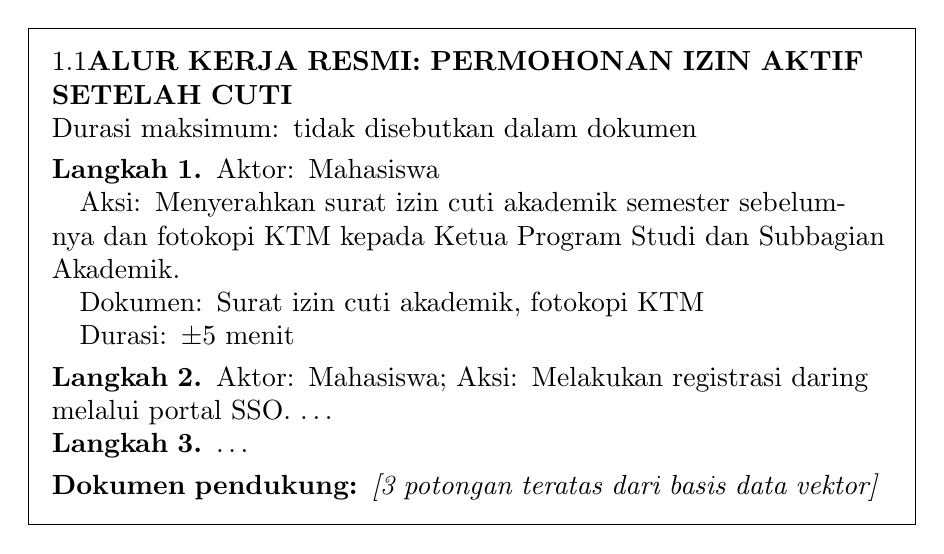
\begin{tikzpicture}
\node[draw, inner sep=3mm, text width=0.88\linewidth, align=left, font=\normalsize, execute at begin node=\setstretch{1.1}] {%
\textbf{ALUR KERJA RESMI: PERMOHONAN IZIN AKTIF SETELAH CUTI}\\
Durasi maksimum: tidak disebutkan dalam dokumen\\[3pt]
\textbf{Langkah 1.} Aktor: Mahasiswa\\
\hspace*{1em}Aksi: Menyerahkan surat izin cuti akademik semester sebelumnya dan fotokopi KTM kepada Ketua Program Studi dan Subbagian Akademik.\\
\hspace*{1em}Dokumen: Surat izin cuti akademik, fotokopi KTM\\
\hspace*{1em}Durasi: $\pm$5 menit\\[3pt]
\textbf{Langkah 2.} Aktor: Mahasiswa; Aksi: Melakukan registrasi daring melalui portal SSO. \dots\\
\textbf{Langkah 3.} \dots\\[3pt]
\textbf{Dokumen pendukung:} \textit{[3 potongan teratas dari basis data vektor]}};
\end{tikzpicture}
\caption{Contoh Blok Alur Kerja pada \textit{Prompt}}
\label{fig:prompt}
\end{figure}

\subsection{Perancangan Antarmuka Pemrograman Aplikasi}
Komunikasi antara E-Office dan layanan RAG menggunakan REST API dengan format JSON. Rancangan \textit{endpoint} ditunjukkan pada Tabel~\ref{tab:api}.

\begin{table}[htbp]
\caption{Rancangan \textit{Endpoint} REST API}
\label{tab:api}
\centering\tabsetup
\begin{tabularx}{\linewidth}{|C{0.6cm}|C{1.4cm}|L{4.2cm}|Y|}
\hline\hdr
\hrow\textbf{No} & \textbf{Metode} & \textbf{Endpoint} & \textbf{Fungsi} \\\hline
1 & POST & \code{/api/chat} & Mengirim pertanyaan dan menerima jawaban beserta sumber (E-Office) \\\hline
2 & GET & \code{/api/chat/history} & Mengambil riwayat percakapan pengguna (E-Office) \\\hline
3 & GET & \code{/api/letters/status} & Mengambil status surat milik pengguna (E-Office, dipanggil layanan RAG) \\\hline
4 & POST & \code{/rag/answer} & Menjalankan alur LangGraph untuk satu pertanyaan (layanan RAG) \\\hline
5 & POST & \code{/rag/reindex} & Membangun ulang graf alur kerja dan indeks vektor (layanan RAG, khusus admin) \\\hline
6 & GET & \code{/rag/health} & Memeriksa ketersediaan layanan RAG dan Ollama \\\hline
\end{tabularx}
\end{table}

\subsection{Perancangan Basis Data}
Basis data PostgreSQL E-Office ditambah dua tabel untuk menyimpan percakapan. Rancangan tabel ditunjukkan pada Tabel~\ref{tab:db}.

\begin{table}[htbp]
\caption{Rancangan Tabel Percakapan}
\label{tab:db}
\centering\tabsetup
\begin{tabularx}{\linewidth}{|C{0.6cm}|L{2.8cm}|L{3.0cm}|Y|}
\hline\hdr
\hrow\textbf{No} & \textbf{Tabel} & \textbf{Kolom} & \textbf{Keterangan} \\\hline
1 & \code{chat\_sessions} & \code{id}, \code{user\_id}, \code{created\_at} & Sesi percakapan milik pengguna \\\hline
2 & \code{chat\_messages} & \code{id}, \code{session\_id}, \code{role}, \code{content}, \code{sop\_id}, \code{route}, \code{latency\_ms}, \code{prompt\_tokens}, \code{created\_at} & Pesan pengguna dan asisten beserta SOP terpilih dan data kinerja \\\hline
\end{tabularx}
\end{table}

% ---------------------------------------------------------------------
\section{Implementasi}
\label{sec:implementasi}
Mesin \wgr{} diimplementasikan dalam Python dengan LangChain, LangGraph, NetworkX, dan Chroma, kemudian disajikan sebagai layanan REST. Implementasi melanjutkan kode penelitian pendahuluan dengan memindahkan setiap tahap ke simpul LangGraph. Rancangan fungsi pemilih SOP berdasarkan Persamaan~\ref{eq:skor} ditunjukkan pada Source Code~\ref{src:selector}.

\begin{sourcecode}{Rancangan fungsi pemilih SOP berbasis aturan}{src:selector}
def score(q: str, sop: dict) -> int:
    q = q.lower()
    s = 15 if sop["title"].lower() in q else 0
    for alias in sop["aliases"]:
        if alias in q:
            s += 8
        else:
            s += 2 * sum(w in q for w in alias.split() if len(w) > 2)
    if any(cue in q for cue in PROCEDURAL_CUES):
        words = {w for w in q.split() if len(w) > 4}
        s += sum(bool(words & set(st["action"].lower().split()))
                 for st in sop["steps"])
    return s

def select_sop(state: dict) -> dict:
    best = max(SOPS, key=lambda p: score(state["question"], p))
    s = score(state["question"], best)
    return {"sop_id": best["id"] if s >= 3 else None, "score": s}
\end{sourcecode}

Lingkungan implementasi ditunjukkan pada Tabel~\ref{tab:lingkungan}.

\begin{table}[htbp]
\caption{Lingkungan Implementasi}
\label{tab:lingkungan}
\centering\tabsetup
\begin{tabularx}{\linewidth}{|C{0.6cm}|L{4.0cm}|Y|}
\hline\hdr
\hrow\textbf{No} & \textbf{Komponen} & \textbf{Spesifikasi} \\\hline
1 & Perangkat keras & {[}diisi: prosesor, RAM, GPU server lokal{]} \\\hline
2 & Bahasa pemrograman & Python (mesin RAG), TypeScript (E-Office) \\\hline
3 & Mesin RAG & LangChain, LangGraph, NetworkX, Chroma, FastAPI \\\hline
4 & Model & \texttt{gemma4:e2b} melalui Ollama; \textit{embedding} \texttt{all-indo-e5-small-v4} \\\hline
5 & E-Office & Next.js, Bun, Elysia, PostgreSQL \\\hline
\end{tabularx}
\end{table}

% ---------------------------------------------------------------------
\section{Pengujian dan Evaluasi}
\label{sec:pengujian}
Subbab ini membahas sistem pembanding, prosedur evaluasi kualitas jawaban, pengujian \textit{black-box}, dan pengukuran efisiensi.

\subsection{Sistem Pembanding}
Sistem yang dibandingkan dalam evaluasi kualitas jawaban ditunjukkan pada Tabel~\ref{tab:sistem}. Seluruh sistem menggunakan model \textit{embedding}, parameter \textit{chunking}, basis data vektor, generator, dan templat \textit{prompt} yang sama agar perbedaan hasil hanya berasal dari cara konteks disusun.

\begin{table}[htbp]
\caption{Sistem Pembanding}
\label{tab:sistem}
\centering\tabsetup
\begin{tabularx}{\linewidth}{|C{0.6cm}|L{3.8cm}|Y|}
\hline\hdr
\hrow\textbf{No} & \textbf{Sistem} & \textbf{Konteks yang Diberikan kepada LLM} \\\hline
1 & LLM saja & Tanpa konteks; mengukur pengetahuan bawaan model \\\hline
2 & Naive RAG & Tiga potongan teratas hasil temu kembali padat \\\hline
3 & GraphRAG entitas & Tripel entitas satu lompatan ditambah tiga potongan teratas \\\hline
4 & \wgr{} & Blok alur kerja SOP terpilih ditambah tiga potongan pendukung \\\hline
5 & \textit{Selection-Matched Text} & Teks asli SOP terpilih ditambah tiga potongan pendukung (ablasi) \\\hline
6 & Konteks penuh & Seluruh 7 SOP \\\hline
7 & LightRAG & Graf entitas-relasi yang dibangun otomatis dengan LLM \parencite{guo2024lightrag} \\\hline
\end{tabularx}
\end{table}

Sistem nomor 1 sampai 6 mengikuti rancangan penelitian pendahuluan \parencite{wiratama2026procedure}, sedangkan LightRAG ditambahkan dalam skripsi ini untuk menguji apakah keunggulan \wgr{} tetap berlaku terhadap GraphRAG otomatis, bukan hanya terhadap graf entitas yang disusun manual.

\subsection{Prosedur Evaluasi Kualitas Jawaban}
Evaluasi kualitas jawaban dilakukan dengan langkah-langkah sebagai berikut:
\begin{enumerate}
\item Menjalankan setiap sistem pada 40 pertanyaan benchmark dengan temperatur generator 0.
\item Menghitung KFR dan ROUGE pada 35 pertanyaan yang dapat dijawab, cakupan langkah, TIR, dan AMR pada 11 pertanyaan prosedural, serta akurasi penolakan pada 5 pertanyaan di luar cakupan.
\item Memeriksa secara manual sampel baris penyelarasan langkah untuk mengukur kesesuaian penilai otomatis dengan penilaian manusia.
\item Menghitung \textit{faithfulness} dan \textit{answer relevancy} RAGAs sebagai bukti pendukung.
\item Menguji perbedaan antarsistem dengan uji Wilcoxon berpasangan dan koreksi Holm-Bonferroni.
\item Mengulangi evaluasi dengan satu LLM lokal pembanding untuk menguji kestabilan hasil terhadap pilihan generator.
\end{enumerate}

\subsection{Pengujian Black-Box}
Pengujian \textit{black-box} dilakukan untuk setiap kebutuhan fungsional pada Tabel~\ref{tab:fungsional}. Contoh rancangan skenario uji ditunjukkan pada Tabel~\ref{tab:blackbox}; daftar lengkapnya disajikan pada Lampiran 2.

\begin{table}[htbp]
\caption{Contoh Rancangan Skenario Pengujian \textit{Black-Box}}
\label{tab:blackbox}
\centering\tabsetup
\begin{tabularx}{\linewidth}{|C{0.6cm}|C{1.2cm}|L{4.0cm}|Y|}
\hline\hdr
\hrow\textbf{No} & \textbf{Kode} & \textbf{Skenario} & \textbf{Hasil yang Diharapkan} \\\hline
1 & F-02 & Mengirim ``bagaimana cara cuti kuliah?'' & SOP Izin Cuti Akademik terpilih \\\hline
2 & F-03 & Menanyakan prosedur legalisir ijazah & Enam langkah tampil berurutan dengan aktor yang benar \\\hline
3 & F-04 & Menanyakan aturan wisuda yang tidak ada dalam SOP & Sistem menolak dengan pesan bahwa informasi tidak tersedia \\\hline
4 & F-05 & Menanyakan ``surat saya sudah sampai mana?'' & Status surat terakhir pengguna, tahap berikutnya, dan aktornya tampil \\\hline
5 & F-07 & Membuka kembali halaman percakapan & Riwayat percakapan sebelumnya tampil \\\hline
\end{tabularx}
\end{table}

\subsection{Pengukuran Efisiensi}
Efisiensi diukur dari jumlah token \textit{prompt}, jumlah pemanggilan LLM, dan waktu respons untuk setiap pertanyaan. Waktu respons diukur dari saat \textit{backend} E-Office menerima pertanyaan sampai jawaban dikirim kembali, sehingga mencakup waktu temu kembali, pemanggilan LLM, dan komunikasi antarlayanan.

% ---------------------------------------------------------------------
\section{Jadwal Penelitian}
\label{sec:jadwal}
Jadwal pelaksanaan penelitian ditunjukkan pada Tabel~\ref{tab:jadwal}. % TODO: sesuaikan dengan tanggal seminar proposal

\begin{table}[htbp]
\caption{Jadwal Penelitian}
\label{tab:jadwal}
\centering\tabsetup
\newcommand{\x}{\cellcolor{g55}}
\begin{tabular}{|c|L{5.0cm}|C{1.05cm}|C{1.05cm}|C{1.05cm}|C{1.05cm}|C{1.05cm}|C{1.05cm}|}
\hline\hdr
\textbf{No} & \textbf{Kegiatan} & \textbf{Okt} & \textbf{Nov} & \textbf{Des} & \textbf{Jan} & \textbf{Feb} & \textbf{Mar} \\\hline
1 & Studi literatur dan pengumpulan data & \x & \x & & & & \\\hline
2 & Analisis kebutuhan & \x & \x & & & & \\\hline
3 & Perancangan sistem & & \x & \x & & & \\\hline
4 & Implementasi mesin RAG dan integrasi E-Office & & & \x & \x & & \\\hline
5 & Pengujian dan evaluasi & & & & \x & \x & \\\hline
6 & Penyusunan laporan & \x & \x & \x & \x & \x & \x \\\hline
\end{tabular}
\end{table}
